\documentclass[12pt]{article}
\usepackage[latvian]{babel}
\usepackage[left=3cm,top=2cm,right=2cm,bottom=2cm]{geometry}
\usepackage{graphicx}
\usepackage{float}
\usepackage{titletoc}
\usepackage{caption}
\usepackage[backend=bibtex]{biblatex}
\usepackage{sectsty}
\usepackage{biblatex}
\usepackage{chngcntr}
\counterwithin{figure}{section}
\counterwithin{table}{section}
\addbibresource{references.bib}
\sectionfont{\centering}
\subsectionfont{\centering}
\subsubsectionfont{\centering}
\title{Music Overflow}

\addto\captionslatvian{\renewcommand{\figurename}{Attēls}}

\begin{document}

\begin{titlepage}
	\begin{center}
		\vspace*{1cm}
 
       LATVIJAS UNIVERSITĀTE \\
       DATORIKAS FAKULTĀTE
 
       \vspace{3cm}
 
       \textbf{\Huge{MUSIC OVERFLOW}}
       
       \vspace{5cm}
       \large{NOSLĒGUMA DARBS\\
       PROGRAMMINŽENIERIJĀ}
       
     \end{center}
       \vfill
       
       \begin{flushright}
       \textbf{Autori}:\\
		Deina Banka\\
		Edgars Lauks\\
		Jeļizaveta Zaharova\\
		Margarita Parhomenko\\
		Toms Bēmis\\
		\bigskip
		\textbf{Darba zinātniskais vadītājs}:\\ Doc. Dr. Dat. Maksims Kravcevs
       \end{flushright}
       
		\vspace{1cm}       
       
       \begin{center}
       \textbf{RĪGA, 2020}
       \end{center}
 
\end{titlepage}

\begin{center}
\textbf{\large Anotācija}
\end{center}

\indent Darba nosaukums: ``Music Overflow''.\\
\indent Darba veids: programmatūras prasības specifikācija (PPS).\\

Šī darba mērķis ir izveidot programmas prasības specifikāciju (PPS), kas apraksta sistēmu ``Music Overflow''.
Sistēma ``Music Overflow'' ir lietotne, kura palīdz lietotājiem iegūt orģinālo dziesmas nosaukumu, ja ir zināma tikai melodija, uzklausot citu lietotāju minējumus. ``Music Overflow'' sniedz iespēju veidot jautājumus, kuros iespējams atdarināt melodiju, kas dotu pietiekošu informāciju par orģinālo dziesmu, kā arī apmainīties ar sevis radītām melodijām un komentāriem par tām. Sistēma arī glabā lietotāju ievadītās melodijas, datus un saites uz attiecīgo skaņdarbu, ja atrasts. \\
\indent Rezultātā izstrādāta programmas prasības specifikācija, ar kuru palīdzību var izveidot funkcionējošo sistēmu ``Music Overflow''. \\
\indent Darbs sastāv no 3 daļām. Tā pirmajā daļā ir sistēmas lietotāju apraksts un tās projektējums, sistēmas ierobežojumi, pieņēmumi un atkarības. Otrajā daļā ir datu bāzes apraksts un funkcionālās un nefunkcionālās prasības sistēmai. Trešajā daļā doti datu bāzes, funkciju, un lietotāja saskarņu projektējumi. \\
\indent Darbs kopumā izklāstīts 25 lappusēs, tajā iekļautas 2 tabulas un 16 attēli.  Darbā izmantoti 8 literatūras avoti un pievienoti 3 pielikumi.

Atslēgas vārdi: mūzika, melodija, dziesma.

\pagebreak

\begin{center}
\textbf{\large Abstract}\\
\end{center}

\indent Project name: ``Music Overflow''\\
\indent Project type: Software Requirements Specification (SRS)\\

Goal of this project is to create a software requirements specification, which describes the system ``Music Overflow''. System ``Music Overflow'' is an application, which helps users to find the title of an original song, by knowing only the melody, by reading the guesses of other users. ``Music Overflow'' offers to create questions, in which it is possible to recreate a melody, which would give enough information about the original song, and to create original melodies to share and give comments about. System also stores user created melodies, data and links to the correct composition, if found.\\
\indent As a result a systems requirement specification has been designed, with which a functional system ``Music Overflow'' can be developed.\\
\indent The project consists of 3 parts. The first part consists of description of the system's users and it's design, limitations of the system, assumptions and dependencies. Second part consists of description of the database and functional and non-functional requirements for the system. Third part consists of database, function and user interface designs.\\
\indent The project consists of 25 pages, it has 2 tables and 16 images. 8 sources have been used and 3 attachments added.\\
\indent Keywords: music, melody, song.

\pagebreak

\tableofcontents

\pagebreak

\section*{Ievads}
\addcontentsline{toc}{section}{Ievads}

\textbf{Nolūks}

Šī programmatūras prasību specifikācija (PPS) ir izstrādāta un paredzēta lietotnes ``Music Overflow'' prasību aprakstīšanai.
Tās nolūks ir precīzi aprakstīt būtiskākās programmatūras darbības funkcijas, to prasības un iespējas, kā arī lietotāja saskarņu prasības, lai pēc specifikācijas izstrādes ir iespējama tālāka lietotnes galīgā izstrāde lietotājam izmantojamā veidā.
Lietotnes nolūks ir palīdzēt atrast dziesmas nosaukumu, no kuras atceras tikai melodijas daļu.
Atbilstoši šai specifikācijai tiks izstrādāta sistēma. Šis dokuments ir savstarpēja vienošanās starp pasūtītāju un izpildītāju. Šajā prasību specifikācijā tiek noformulētas sistēmas prasības un raksturota funkcionalitāte.

\textbf{Darbības sfēra}

Sistēma ``Music Overflow'' ir lietotne, kura glabā lietotāju ievadītās melodijas, datus un saites uz attiecīgo skaņdarbu. Šī lietotne sniedz lietotājiem iespēju veidot jautājumus, kuros iespējams atdarināt mūzikas ierakstu, ievadot ritmu, kas dod pietiekošu informāciju par orģinālo dziesmu, kā arī apmainīties ar sevis radītām melodijām un komentāriem par tām.


\textbf{Saistība ar citiem dokumentiem}

Dokumenta noformēšanā ievērotas standarta LVS 68:1996 ``Programmatūras prasību specifikācijas ceļvedis'' prasības.

\textbf{Pārskats}\\
Dokuments sastāv no ievada, 3 nodaļām un pielikumiem:
\begin{itemize}
\item Pirmajā nodaļā tiek izklāstīts par vispārējo programmas aprakstu, esošo stāvokli, sistēmas ierobežojumiem, kā arī atkarības, no citiem faktoriem;
\item Otrajā nodaļā tiek norādītas funkcionālās un nefunkcionālās prasības uz izstrādājamo programmu;
\item Trešajā nodaļā ir dots programmatūras projektējuma apraksts, izklāstot to datu bāzes, funkciju un lietotāju saskarņu projektējumos;
\item Pielikumi sastāv no nodaļu papildinošas informācijas.
\end{itemize}

\pagebreak

\section*{Apzīmējumu saraksts}
\addcontentsline{toc}{section}{Apzīmējumu saraksts}

\begin{itemize}
\setlength{\itemsep}{0em}
\item Atbilde - Lietotāja ievadīts teksts, kas referencē uzdotu jautājumu.\\
Komentārs - Lietotāja ievadīts teksts, kas referencē kādu atbildi par uzdoto jautājumu.\\
Vērtējums - Lietotāju atzinums par to, cik pareiza vai nepareiza ir kāda atbilde.\\
\item URL - (angļu val.)``Unified Resource Locator'' - ``Vienotais Resursu Vietrādis'' jeb tīmekļa adrese.\cite{URL}\\
\item Oauth - atvērtais standarts autorizācijas resursu deleģēšanai.\cite{Oauth}\\
\item MVC - (angļu val.)``Model-View-Controller'' - ``Modelis-Skats-Kontrolieris'' ir projektēšanas šablons, kur programmatūra ir sadalīta trijās patstāvīgās komponentēs, katra ar savu uzdevumu un mērķi.\cite{C2}\\
\item HTML - (angļu val.)``HyperText Markup Language'' - ``Hiperteksta iezīmēšanas valoda'' ir standarta iezīmēšanas valoda, kas izstrādāta tīmekļa lappušu attēlošanai pārlūkprogrammās.\cite{HTML}\\
\item SQL - (angļu val.)``Structured Query Language'' - ``Strukturēto Vaicājumu Valoda'' ir vaicājumu valoda, kas paredzēta datu manipulēšanai relāciju datubāžu pārvaldības sistēmās.\cite{SQL}\\
\item SQL injekcija - uzbrukuma veids, kurā uzbrucējs datu ievades laukā ievada datu bāzes vaicājumus, kurus tā izpildīs.\cite{injection}\\
\item XSS - (angļu val.)``Cross Site Scripting'' - ``Starpvietņu skriptošana'' ir uzbrukuma veids, kurā uzbrucējs var likt citu tās pašas mājaslapas lietotāju pārlūkprogrammām izpildīt uzbrucēja rakstītu kodu.\cite{XSS}\\
\item CSRF - (angļu val.)``Cross Site Request Forgery'' - ``Starpvietņu Pieprasījumu Viltošana'' ir uzbrukuma veids, kurā uzbrucēja izveidota vietne sūta pieprasījumus uz citu vietni, kamēr abas šīs vietnes ir atvērtas kāda lietotāja pārlūkprogrammā.\cite{CSRF}\\
\end{itemize}

\pagebreak

\section{Vispārējais apraksts}

\subsection{Esošā stāvokļa apraksts}

Jaunas tīmekļa lietojumprogrammas izstrāde, mūzikas ierakstu atdarināšanai un orģinālo autoru un autordarbu identificēšanai.

\subsection{Pasūtītājs}

Sistēma aprakstīta pēc studentu grupas iniciatīvas programminženierijas kursa ietvaros.

\subsection{Produkta perspektīva}

Uzturēt saiti starp sistēmas lietotājiem un informāciju mūzikas datubāzēs. Ērti izveidot melodijas, piemeklēt tām esošus skaņdarbus, dalīties ar mūzikas ierakstiem un viedokļiem par tiem vienotā integrālā sistēmā.

\subsection{Darījumprasības}
\begin{itemize}
\item Sniegt lietotājiem iespēju veidot jautājumus, kuros iespējams atdarināt mūzikas ierakstu, kas dod pietiekošu informāciju par orģinālo dziesmu.
\item Piedāvāt lietotājiem atrisināt citu lietotāju uzdotos jautājumus, lai veiksmīgi atrastu ieraksta autoru vai dziesmas nosaukumu.
\item Informēt lietotājus, ļaut tiem sazināties savā starpā un paziņot par veiksmīgi atrastu izpildītāju un dziesmu.
\item Dot iespēju mūzikas izpildītājiem tikt atpazītiem starp patērētājiem, neaizskarot autortiesības.
\item Sniegt lietotājiem iespēju dalīties ar mūziku caur Facebook.
\end{itemize}

\subsection{Sistēmas lietotāji}

Lietojumprogramma pieejama tikai izmantojot pārlūkprogrammu. Lietotājam ir nepieciešamas pamatzināšanas mūzikā, kā arī ir nepieciešama prasme darbam ar datoru un ar uzstādīto interneta pārlūkprogrammu. Administratoram nav nepieciešamas specifiskas mūzikas zināšanas, bet ir nepieciešamas datu apstrādes zināšanas. Lietotāji sadalīti pa 3 lomām, kuras var aplūkot ~\ref{fig:lomas} tabulā un ~\ref{fig:dpd_0} diagrammā.\\

\begin{center}
\begin{tabular}{|c|c|}
\hline
Administrators & Jauna lietotāja pievienošana  \\
& Lietotāja visas informācijas izdzēšana \\
& Komentāru rediģēšana \\
\hline
Reģistrēts lietotājs & Ritma ievadīšana \\
& Nošu pievienošana \\
& Konta dzēšana \\
& Dalīšanās ar savu melodiju\\
\hline
Nereģistrēts lietotājs & Konta izveidošana \\
& Ritma ievadīšana \\
& Nošu pievienošana \\
\hline
\end{tabular}
\captionof{table}{Lietotāju lomas}
\label{fig:lomas}
\end{center}

\begin{figure}[H]
\begin{center}
		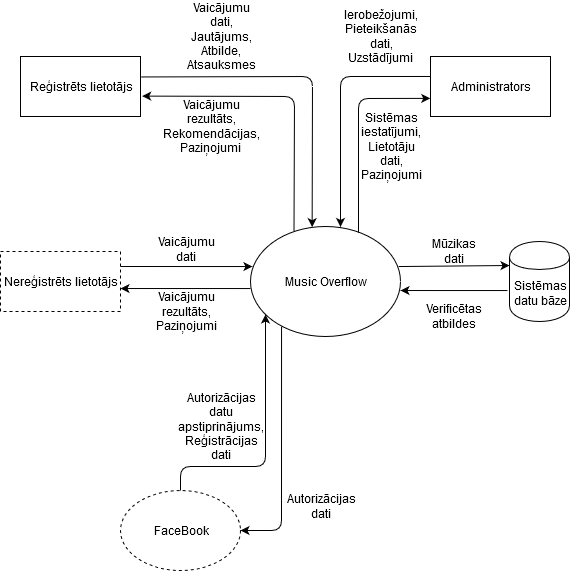
\includegraphics[scale=0.5]{DPD0.png}
		\caption{Datu plūsmas 0. līmeņa diagramma}
		\label{fig:dpd_0}
\end{center}
\end{figure}

\subsection{Vispārējie ierobežojumi}

\begin{itemize}
\setlength{\itemsep}{0em}
\item Sistēmas darbināšanai jābūt bez instalēšanas un izmantojot pārlūkprogrammu.
\item Sistēmas darbībai jābūt atbalstītai uz trim populārākajām pārlūkprogrammām: FireFox, Chrome, Safari.
\item Prasību apkopošanas laikā netika identificēti faktori, kuru izmaiņas var atstāt iespaidu uz prasību realizāciju.
\item Nepieciešams aizsargāt autortiesības par oriģinālo melodiju.
\item Laika ierobežojums melodijas ievadīšanai.
\end{itemize}

\subsection{Pieņēmumi un atkarības}

Pieeja publicēt jautājumus nepieciešama autentifikācija izmantojot trešo personu autentifikācijas informāciju, vai izveidoto kontu lietojumprogrammā. Lietotājam nepieciešams veids kā atskaņot audio. Pārlūkprogrammai nepieciešams HTML tehnoloģijas atbalsts, priekš lietotāja ievades rīka mūzikas atdarināšanai.

\pagebreak

\section{Programmatūras prasību specifikācija}

\subsection{Konceptuālais datu bāzes apraksts}

``Music Overflow'' programmatūras datu bāzē pastāv 6 entītijas: lietotājs, loma, jautājums, mūzikas
atdarinājums, atbilde un komentārs (skat. ~\ref{fig:db_konceptualais} attēlu). Lietotājs ir sistēmas lietotājs, kas ir reģistrēts datu bāzē. Tas
atšķiras no nereģistrēta lietotāja ar iespēju autentificēties un iespēju veidot saturu vietnē.
Lietotājiem tiek piešķirta loma. Šis atribūts nosaka, vai lietotājs ir parasts lietotājs vai administrators,
kam ir privilēģijas pār lietotāja veidoto saturu vietnē. Visiem lietotājiem ir iespēja uzdot vairākus
jautājumus. Jautājumi satur tekstuālu informāciju par meklējamo mūzikas ierakstu. Tiem arī ir
atribūts statuss, kas norāda vai jautājumam ir sniegta atbilde, kas atzīta par pareizu. Šādā veidā tiek
noslēgta diskusija ar jautātāju. Jautājumam var būt arī pievienots mūzikas atdarinājums, kas ir
lietotāja ievadīta informācija par attiecīgā mūzikas ieraksta melodiju. Vēl viena svarīga entītija ir
atbilde, kas ir piesaistīta vienam jautājumam. Līdzīgi kā jautājumam, šai entītijai ir atribūti teksts un
statuss. Papildus atbildei ir vērtējums, kas atspoguļo cik lietderīga atbilde ir bijusi citiem
lietotājiem. Katrai atbildei var būt vairāki komentāri, kuros lietotāji diskutē par atbildi. Komentāram
ir tie paši atribūti, kas atbildei, izņemot statusu.

\begin{figure}[H]
\begin{center}
	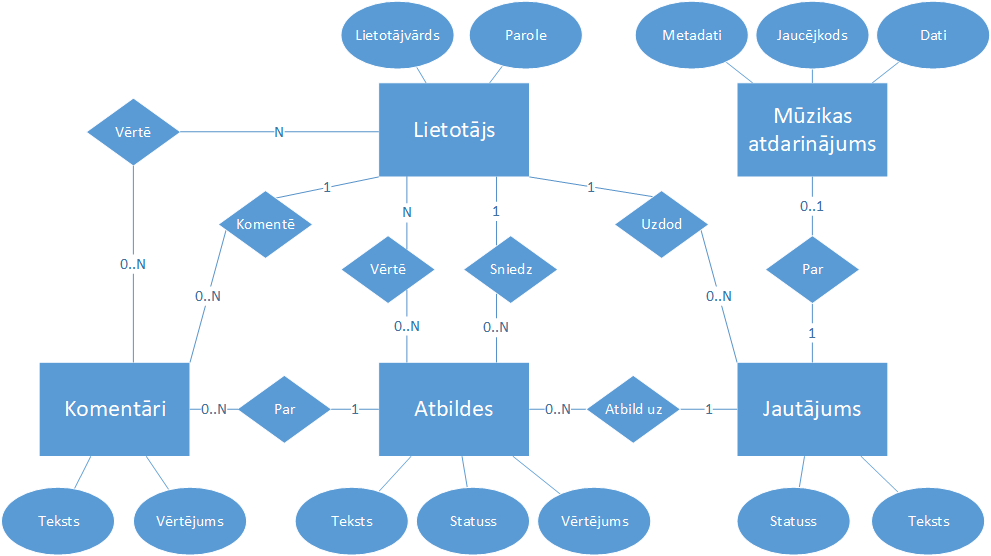
\includegraphics[scale=0.5]{DB_concept.png}
	\caption{Datubāzes konceptuālais modelis}
	\label{fig:db_konceptualais}
\end{center}
\end{figure}

\subsection{Funkcionālās prasības}

\subsubsection{Vispārējās nodaļas, kas saistītas ar funckiju aprakstīšanu}

\textbf{Autentifikācija.} Sistēmā lietotājiem ir iespēja veidot saturu, bet pastāv ierobežojums, ka lietotājiem ir jāautentificējas. Tas nodrošina, ka vietnē netiek ļaunprātīgi publicēts saturs, kuram nav nozīmes. Lietotājiem piemīt unikāls lietotājvārds un parole, kuru izmanto, lai autentificētos. Programmatūra loģiski nosaka, kuras funkcijas attiecīgajam lietotājam ir pieejamas.\\
\indent \textbf{Publikāciju atspoguļošana.} ``Music Overflow'' komponentu shēma (skat. ~\ref{fig:dpd_1} attēlu) paredz, ka lietotāji var iegūt vietnē publicēto saturu pēc tā pieprasījuma. Tas tiek panākts ar MVC programmatūras projektējuma veidu, un šis projektējums sniedz iespēju entītijas uzskatīt par objektu kopām. Šīs objektu kopas ir iespējams atlasīt un kārtot, kas ir lietderīgi lietotājam. Piemēram, lai lietotājam atspoguļotu vispopulārākās atbildes uz jautājumu, tiek izmantots vaicājums par atbildēm, kas attiecas un konkrētu jautājumu. Kad vaicājums atgriež sarakstu, tad saraksts tiek kārtots pēc vērtējuma lauka dilstošā secībā. Rezultējošais saraksts tiek izmantots, lai uzģenerētu HTML, kas lietotājam atspoguļo aktuālu informāciju. 

\subsubsection{Funkciju sadalījums pa moduļiem/komponentiem}

``Music Overflow'' funkcijas ir sadalītas trīs moduļos: jautājumu un atbilžu, mūzikas atdarināšanas un lietotāju modulī. Sistēmas lietotāji ir sadalīti nereģistrētos lietotājos un reģistrētos lietotājos, kur reģistrētie ir sadalīti pēc to lomām sistēmas funkciju izpildē. Nereģistrētiem lietotājiem ir pieejami publicētie jautājumi un iespēja saglabāt savus pierakstīšanās datus datu bāzē, lai kļūtu par reģistrētiem lietotājiem. Reģistrēto lietotāju lomas ir jautātājs, atbildētājs un administrators. Reģistrētajiem lietotāji arī var iegūt sarakstus ar publicētiem jautājumiem un aplūkot to saturu. Jautātājam īpatnēja ir datu plūsma saistībā ar mūzikas atdarināšanas moduļa (skat. ~\ref{fig:dpd_2_1} attēlu) funkcijām, jo lietotāji jautājuma uzdošanas situācijā izmanto rīku mūzikas atdarinājuma izveidei. Turpretim atbildētāji izmanto jautājumu un atbilžu moduli (skat. ~\ref{fig:dpd_2_2} attēlu), lai sniegtu atbildes uz jautājumiem. Papildus atbildētāji vērtē komentārus un atbildes. Administratoram ir pieejamas funkcijas, kas ļauj veikt labojumus reģistrēto lietotāju publicētajā saturā. Informācija datu bāzē ir iedalāma 4 daļās. 3 daļas priekš katra sistēmas moduļa un vēl viena datu bāzes daļa priekš audio fragmentiem, kurus lietotājiem vajag, lai atskaņotu mūzikas atdarinājumus.

\begin{figure}[H]
\begin{center}
	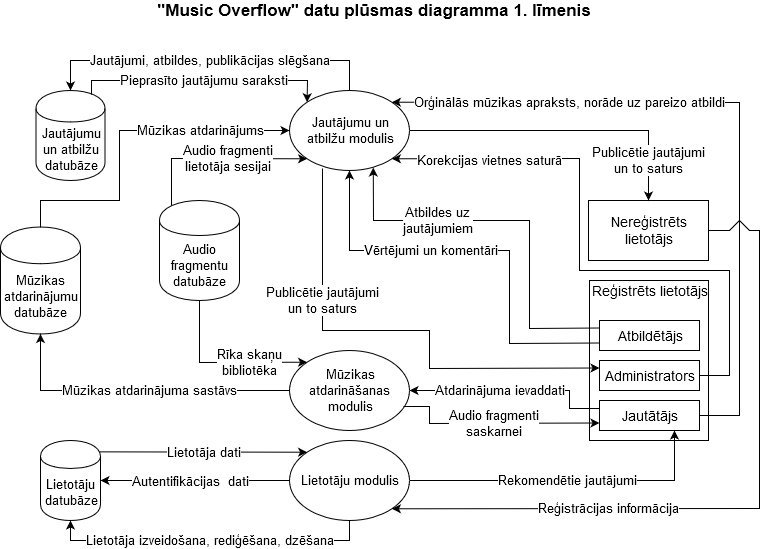
\includegraphics[scale=0.5]{DPD1.png}
	\caption{Datu plūsmas 1. līmeņa diagramma}
	\label{fig:dpd_1}
\end{center}
\end{figure}

\subsubsection{Mūzikas atdarināšanas modulis}

Galvenās sadaļas mūzikas atdarināšanas modulī (skat. ~\ref{fig:dpd_2_1} attēlu) ir jautātājs, kas ievada informāciju, mūzikas atdarinājuma rīks un datubāze, kurā tiek saglabāts objekts. Lai jautātājs izmantotu rīku pilnvērtīgi, ir nepieciešami audio fragmenti, kurus jautātājs klausās un izvērtē, vai ievadītās notis atbilst oriģinālā mūzikas ieraksta melodijai. Lietotājs izmanto rīku, lai ievadītu nošu izkārtojumu, sitienu skaitu un ritmu. Lietotājs papildus ievada tekstuālu informāciju (nosaukumu). Ievadītā informācija tiek nodota apstrādei, kur tiek noteikta informācija par atdarinājumu (ātrums, garums, nošu skaits). Mūzikas atdarinājuma apstrādes funkcijas vēl uzģenerē jaucējkodu, kas nepieciešams jautājumu un atbilžu funkcionalitātei 2.10 ``Jautājumu rekomendācijas'' (skat. pielikumu). Pēc informācijas apstrādes objekts tiek saglabāts kā viens ieraksts datu bāzē.

\begin{figure}[H]
\begin{center}
	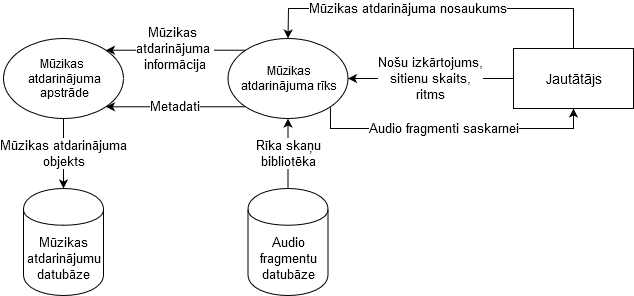
\includegraphics[scale=0.5]{DPD2_1.png}
	\caption{Datu plūsmas 2. līmeņa diagramma mūzikas atdarināšanas modulim}
	\label{fig:dpd_2_1}
\end{center}
\end{figure}

\subsubsection{Jautājumu un atbilžu modulis}

Jautājumu un atbilžu modulis (skat. ~\ref{fig:dpd_2_2} attēlu) satur funkcijas, kuras iespējams iedalīt 3 daļās: jautājumu, atbilžu un vērtējumu un komentāru funkcijas. Jautājumi var saturēt vairākas atbildes un atbildes var saturēt vairākus komentārus. Lai jautājumu atspoguļotu lietotājam, tai skaitā nereģistrētam lietotājam, to nepieciešams apkopot ar attiecīgo mūzikas atdarinājumu, ja tāds pastāv. Vēl viena datu plūsma uz jautātājiem ir rekomendētie jautājumi, kas tiek piedāvāti ņemot vērā iepriekš uzdotos jautājumus. Administratori ietekmē jautājumu sarakstus kas tiek atspoguļoti pārējiem lietotājiem, lai vietnes saturs atbilstu tās noteikumiem par publicējamo saturu. Atbildētāji izmanto atbildes, komentārus un vērtēšanu, lai rosinātu diskusiju par attiecīgo jautājumu. Jautātājam ir iespēja slēgt jautājumu un pasludināt to par atrisinātu, ja tas atzīmē vienu no atbildēm par pareizu.

\begin{figure}[H]
\begin{center}
	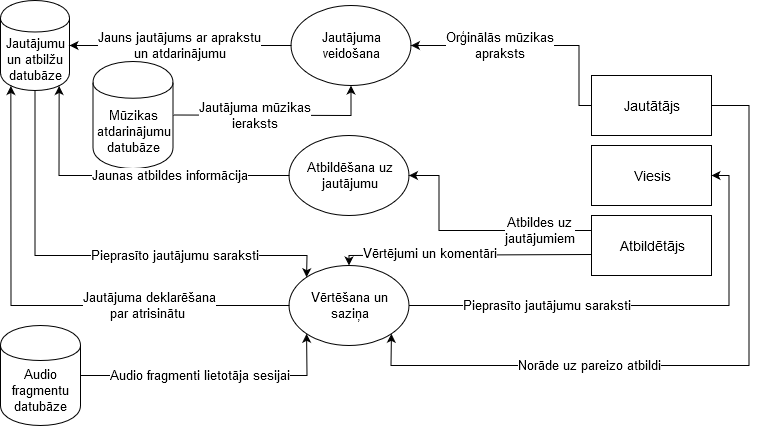
\includegraphics[scale=0.5]{DPD2_2.png}
	\caption{Datu plūsmas 2. līmeņa diagramma jautājumu un atbilžu modulim}
	\label{fig:dpd_2_2}
\end{center}
\end{figure}

\subsubsection{Lietotāju modulis}

``Music Overflow'' lietotāju modulis (skat. ~\ref{fig:dpd_2_3} attēlu) ietver funkcijas, kas saistītas ar lietotāju ielogošanos, reģistrāciju, konta informācijas atspoguļošanu, rediģēšanu un konta dzēšanu. Visas funkcijas neattiecas uz visiem lietotājiem. Lietotājs, kas ir viesis, nav piereģistrējies vietnē. Viesim ir iespēja ievadīt savu pierakstīšanās informāciju, un, ja tā ir derīga, tad attiecīgais lietotājs var izmantot reģistrēta lietotāja privilēģijas. Reģistrētie lietotāji iedalās parastajos lietotājos un administratoros. Šie divi lietotāju veidi var veikt izmaiņas savā norādītajā informācijā, bet visiem lietotājiem ir iespēja aplūkot kāda lietotāja informāciju. Administratoram ir tiesības dzēst reģistrētu lietotāju, ja tas ir pārkāpis attiecīgos vietnes noteikumus. Vietnē ir iespējams pierakstīties izmantojot ``Music Overflow'' autentifikāciju, vai autorizēties Facebook autorizācijas serverī. Ja tiek izmantots ārējais autentifikācijas veids, tad nepieciešamā informācija par lietotāju tiek nodota ``Music Overflow'' serverim.

\begin{figure}[H]
\begin{center}
	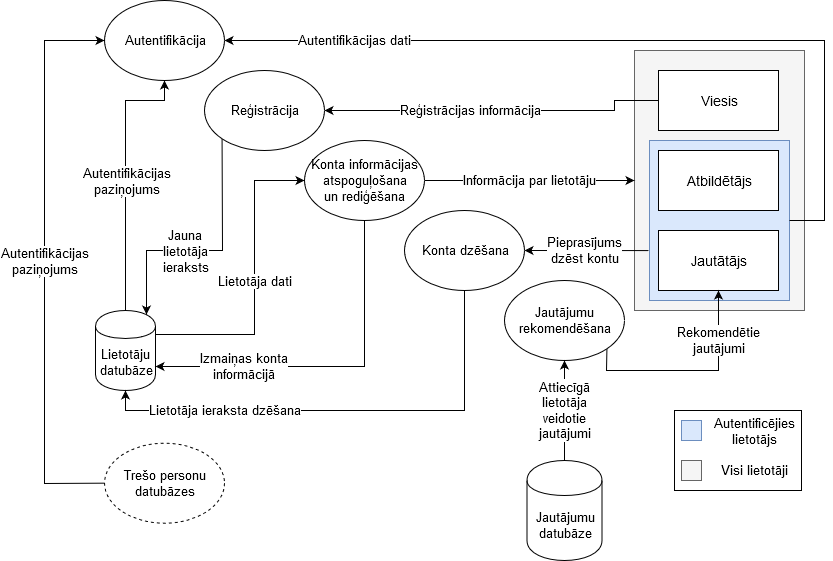
\includegraphics[scale=0.4]{DPD2_3.png}
	\caption{Datu plūsmas 2. līmeņa diagramma lietotāju modulim}
	\label{fig:dpd_2_3}
\end{center}
\end{figure}

\subsection{Nefunkcionālās prasības}

Sistēmai „Music Overflow” ir jānodrošina sekojošās nefunkcionālās prasības:
\begin{itemize}
	\item Mūzikas atdarinājuma rīka saskarnei jābūt intuitīvai un lai izveidotu mūzikas atdarinājumu nav nepieciešama speciālā izglītība;
	\item Sistēmā netiek uzglabāti audio ieraksti, kas nav uzģenerēti ar mūzikas atdarinājuma rīku. Lai nepārkāptu autortiesības, audiālā informācija sistēmā jābūt vispārinātai un nesaistītai ar esošu izpildītāju darbiem;
	\item Izmantojot Facebook autorizāciju no lietotāja tiek ievākta tā pati informācija, kas tiek pieprasīta no ``Music Overflow'' konta īpašnieka;
	\item Lietotāji ar lomu administrators ir tiesīgi izdzēst uzdotos jautājumus un izdzēst lietotājus tikai saskaņā ar ``Music Overflow'' lietošanas noteikumiem;
	\item Lietotāju paroles sistēmas iekšienē uzglabā tikai šifrētā veidā;
	\item Sistēma ir jānodrošina pret SQL injekcijām un XSS un CSRF uzbrukumiem;
	

\end{itemize}

\subsubsection{Veiktspējas prasības}

Sistēmai jāspēj nodrošināt vairāku (vismaz 1000) lietotāju vienlaicīgu sistēmas lietošanu. Apstrādājamo datu apjoms, uz apstrādes ilgumu ierobežojošiem laika limitiem.

\subsubsection{Drošība}

Katram lietotājam būs parole, kura neļaus nepiederošām personām patvaļīgi piekļūt pie sistēmas. Ar autortiesībām aizsargā oriģinālās melodijas autora darbu pret neatļautu lietošanu.

\pagebreak

\section{Programmatūras projektējuma apraksts}

\subsection{Datu bāzes projektējums}

Pārejot no konceptuāla modeli (skat. ~\ref{fig:db_konceptualais} attēlu) uz loģisko modeli, tika analizēti tabulu savstārpējas saites (relācijas): konceptuālajā modelī N:N saites pārveršas uz atsevišķu tabulu loģiskajā modeli (LietotajsKomentarsVertejums, LietotajsAtbildeVertejums). Arī tika analīzēti tabulu atribūti, tika pišķirti Primary key zīmes, Foreign key zīmes.
Savukārt, pārejot no loģiskā modeli uz fizisko modeli tika pievinoti datu tips, ierobežojumi, iestatījumi, saites ar citām entītijām un katra atribūta apraksts (skat. ~\ref{fig:db_logiskais} attēlu).

\begin{figure}[H]
\begin{center}
	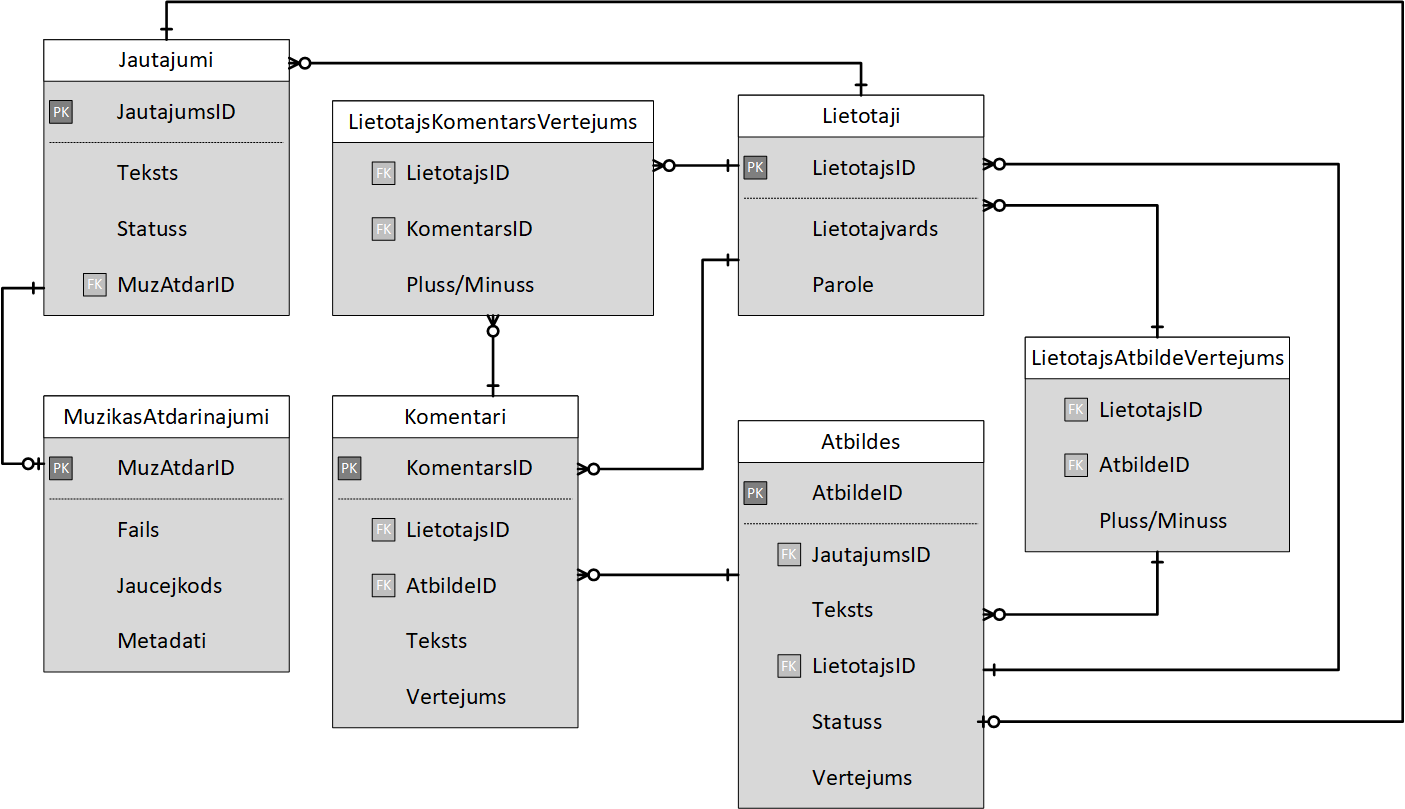
\includegraphics[scale=0.35]{DB_logical.png}
	\caption{Datu bāzes loģiskais modelis}
	\label{fig:db_logiskais}
\end{center}
\end{figure}

\begin{center}
\resizebox{\columnwidth}{!}{\begin{tabular}{|l|l|l|l|}
	\hline
	\textbf{Entītija} & \textbf{Attribūti} & \textbf{Datu tips} & \textbf{Apraksts} \\
	\hline
	\textbf{Lietotāji} & LietotajsID & INT, autoincrement, PK, NOT NULL & Glabājas lietotāja identifikācijas numurs \\
	\cline{2-4}
	& Lietotajvards & nvarchar(30), NOT NULL & Glabājas lietotāja vārds \\
	\cline{2-4}
	& Parole & char(64), NOT NULL & Glabājas SHA256 kodēta lietotāja parole \\
	\hline
	\textbf{Atbildes} & AtbildesID & INT, autoincrement, PK, NOT NULL & Glabājas atbildes identifikācijas numurs \\
	\cline{2-4}
	& Teksts & TEXT, NOT NULL & Glabājas atbildes saturs \\
	\cline{2-4}
	& Statuss & BOOLEAN, NOT NULL & Glabājas atbildes statuss (pareiza/nepareiza), kuru nosaka jautājuma autors \\
	\cline{2-4}
	& Vertejums & INT, NOT NULL & Rādītājs, pēc kura kārtot jautājuma atbildes (var būt negatīvs) \\
	\cline{2-4}
	& JautajumsID & INT, NOT NULL & Atslēga jautājumu, uz kuru dota šī atbilde \\
	\cline{2-4}
	& LietotājsId & INT, NOT NULL & Atslēga uz lietotāju, kurš izveidoja šo atbildi \\
	\hline
	\textbf{LietotajsAtbildeVertejums} & Vertejums & BOOLEAN, NOT NULL & Glabājas lietotāja vērtējums par kādu atbildi (2 varianti: + vai -)\\
	\cline{2-4}
	& LietotajsID & INT, NOT NULL & Atslēga uz lietotāju, kurš veicis šo vērtējumu atbildei\\
	\cline{2-4}
	& AtbildeID & INT, NOT NULL & Atslēga uz atbildi, par kuru lietotājs ir licis vērtējumu\\
	\hline
	\textbf{Komentari} & KomentarsID & INT, autoincrement, PK, NOT NULL & Glabājas komentāra identifikācijas numurs\\
	\cline{2-4}
	& Teksts & TEXT, NOT NULL & Glabājas komentāra saturs\\
	\cline{2-4}
	& Vertejums & INT, NOT NULL & Rādītājs, pēc kura kārtot atbildes komentārus (var būt negatīvs)\\
	\cline{2-4}
	& LietotajsID & INT, NOT NULL & Atslēga uz lietotāju, kurš izveidoja šo komentāru\\
	\cline{2-4}
	& AtbildeId & INT, NOT NULL & Atslēga uz atbildi, kurai tika pievienots šis komentārs\\
	\hline
	\textbf{LietotajsKomentarsVertejums} & Vertejums & BOOLEAN, NOT NULL & Glabājas lietotāja vērtējums par kādu komentāru (2 varianti: + vai -)\\
	\cline{2-4}
	& LietotajsID & INT, NOT NULL & Atslēga uz lietotāju, kurš veicis šo vērtējumu komentāram\\
	\cline{2-4}
	& KomentārsID & INT, NOT NULL & Atslēga uz komentāru, par kuru lietotājs ir licis vēŗtējumu\\
	\hline
	\textbf{MuzikasAtdarinajumi} & MuzikasAtdarID & INT, autoincrement, PK, NOT NULL & Glabājas mūzikas atdarinājuma identifikācijas numurs\\
	\cline{2-4}
	& Fails & varchar(64), NOT NULL & Ceļš uz uzģenerēto skaņdarba failu\\
	\cline{2-4}
	& Jaucejkods & char(64), NOT NULL & Jaucējkods, kas iegūts pēc metadatu apstrādes\\
	\cline{2-4}
	& Metadata & TEXT, NOT NULL & Informācija par lietotāja ievadīto melodiju - ritms, sitienu ilgums, nošu izkārtojums, toņkārta\\
	\hline
	\textbf{Jautajumi} & JautajumsID & INT, autoincrement, PK, NOT NULL & Glabājas jautājuma identifikācijas numurs\\
	\cline{2-4}
	& Teksts & TEXT, NOT NULL & Glabājas jautājuma autora apraksts par oriģinālo dziesmu\\
	\cline{2-4}
	& Statuss & BOOLEAN, NOT NULL & Glabājas jautājuma statuss (atrisināts vai neatrisināts)\\
	\cline{2-4}
	& MuzikasAtdarID & INT & FK, var pastāvēt jautājums bez mūzikas atdarinājuma\\
	\cline{2-4}
	& LietotajsID & INT, NOT NULL & Atslēga uz lietotāju, kurš uzdevis šo jautājumu\\
	\hline
\end{tabular}}
\captionof{table}{Datubāzes fiziskais modelis}
\end{center}

\subsection{Daļējs funkciju projektējums}

Programmai tiks izmantota Klienta-Servera tīkla arhitektūra. Uz servera notiks ievadīto datu apstrāde un mūzikas failu ģenerācija, kā arī datu saglabāšana datubāzē, savukārt klienta pusē notiks ģenerējamās melodijas metadatu izveide (skat. ~\ref{fig:deployment_diagram} attēlu).

\begin{figure}[H]
\begin{center}
	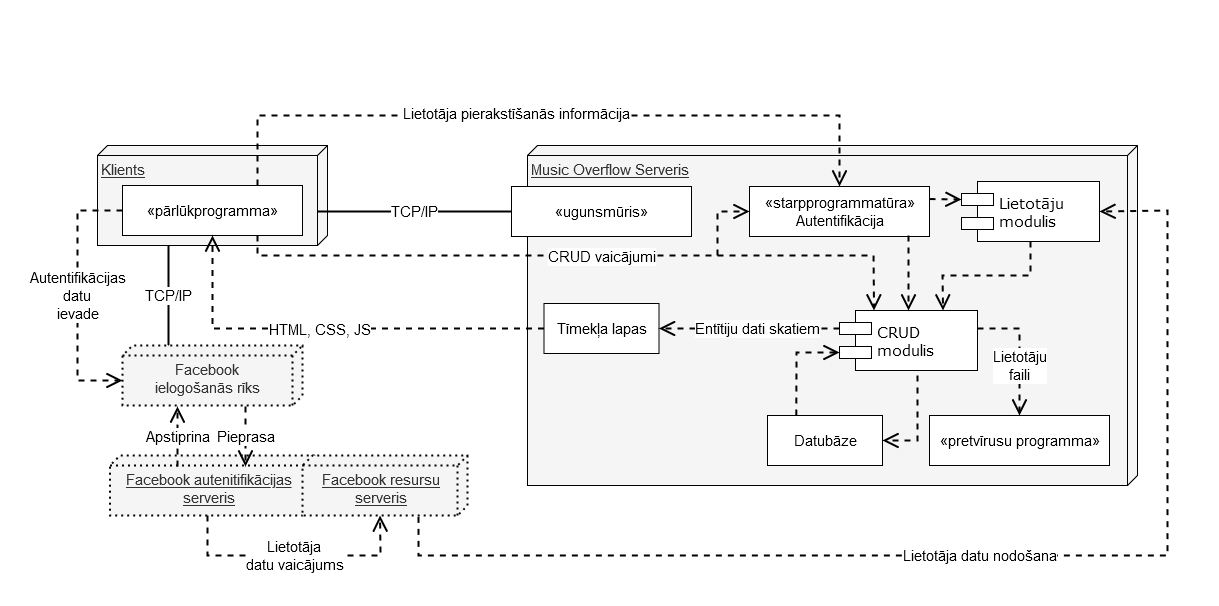
\includegraphics[scale=0.35]{DeploymentDiagram.png}
	\caption{Izvietošanas diagramma}
	\label{fig:deployment_diagram}
\end{center}
\end{figure}

Programmatūra tiks izstrādāta izmantojot ``Modelis-Skats-Kontrolieris'' projektēšanas šablonu. No pārlūkprogrammā ievadītās adreses tiek izsecināts, kurš kontrolieris un kura metode tiek izsaukta. Kontroliera metode apstrādā modeļus, kuri modelē ierakstus datubāzē. Atkarībā no metodes rezultāta, lietotājam tiek parādīta jauna lapa, vai arī tiek izsaukta cita kontroliera metode. Piemērs, kā tas strādā, redzams ~\ref{fig:routing} attēlā. 

\begin{figure}[H]
\begin{center}
	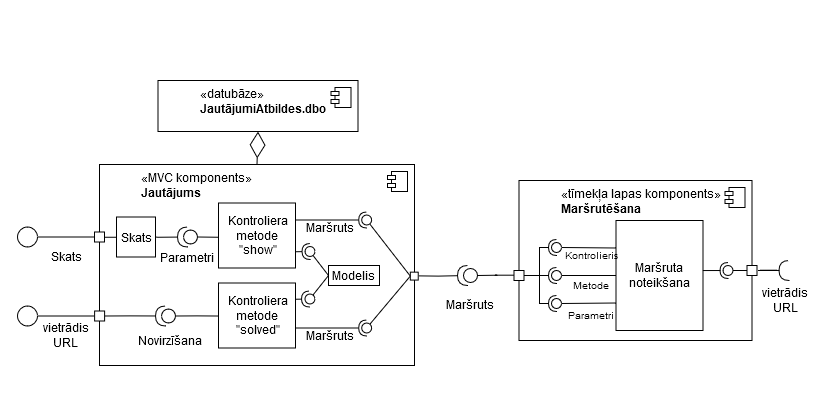
\includegraphics[scale=0.5]{routing.png}
	\caption{Maršrutēšanas diagramma}
	\label{fig:routing}
\end{center}
\end{figure}

Sistēmā ir iespēja pieteikties caur Facebook autentifikāciju (skat. ~\ref{fig:oauth_flow} attēlu). Sistēma ``Music Overflow'' jautā lietotājam pieteikties viņas Facebook kontā, pēc tam, ja autorizācija ir sekmīga, sistēma saņem piekļuves marķieri (token), ar kuru palīdzību iegūt lietotāju datus no Facebook Resursu servera. 

\begin{figure}[H]
\begin{center}
	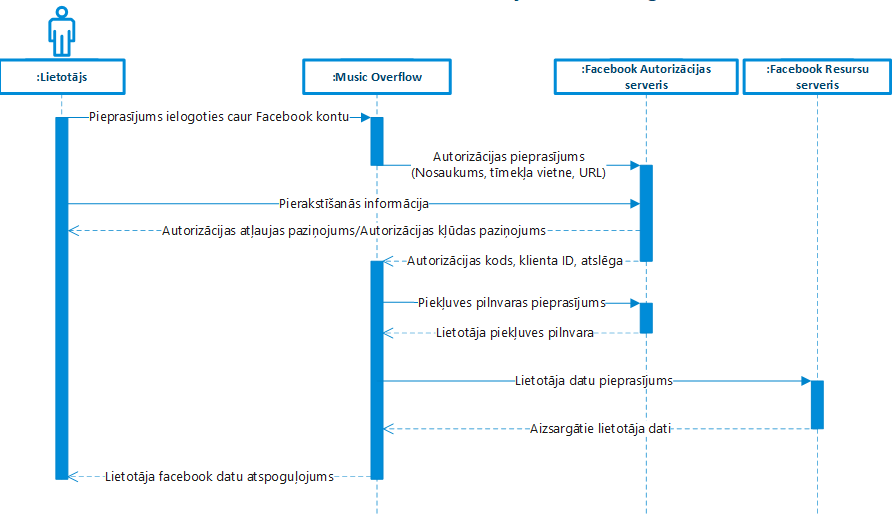
\includegraphics[scale=0.6]{Oauth_flow.png}
	\caption{Autorizācijas diagramma}
	\label{fig:oauth_flow}
\end{center}
\end{figure}

Nozīmīgākā sistēmas funkcija ir mūzikas atdarinājuma izveidošana, jo tās ir sistēmas ``Music Overflow'' galvenā ideja, kura dod lietotājam iespēju izveidot savu mūzikas atdarinājumu, dalīties ar to, vai uzdot par to jautājumu. 
Vispirms lietotājs veido savu atdarinājumu, kuru metode ShowMelody(createdMelody) pārveido par sistēmai saprotāmo objektu, un atgriež skatu, kur atdarinājumu var apskatīt, paklausīties vēlreiz (ShowTheMelodyPage). Šajā brīdī atdarinājumam var pievienot jauno informāciju un/vai pievienot komentāru (skat. ~\ref{fig:activity_diagram} attēlu).

\begin{figure}[H]
\begin{center}
	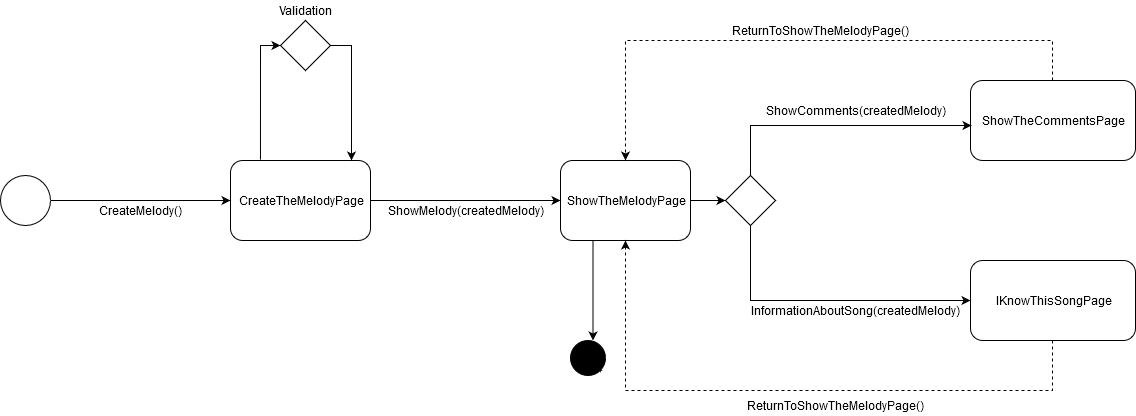
\includegraphics[width=\linewidth,scale=0.5]{ActivityDiagram.png}
	\caption{Aktivitāšu diagramma}
	\label{fig:activity_diagram}
\end{center}
\end{figure}

\subsection{Daļējs lietotāja saskarņu projektējums}

\begin{figure}[H]
\begin{center}
	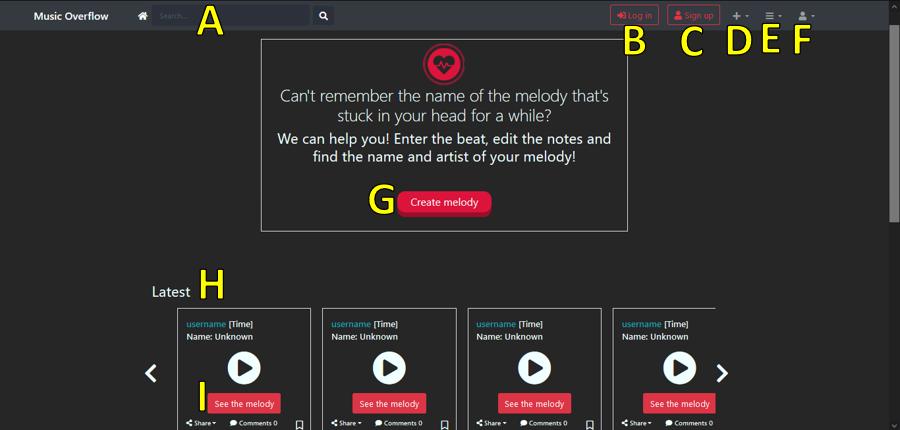
\includegraphics[scale=0.6]{homepage.png}
	\caption{Indeksa lapa}
	\label{fig:homepage}
\end{center}
\end{figure}

Kad lietotājs pirmo reizi ienāk šajā vietnē, būs redzams šāds skats (skat. ~\ref{fig:homepage} attēlu) un pieejamas šādas funkcijas:

\begin{itemize}
	\item A - Jautājuma meklēšanas iespēja;
	\item B - Pilnvarošana sistēmā;
	\item C - Reģistrēšana sistēmā;
	\item D - Izvēlne, kurā var izvelēties izveidot jauno mūzikas atdarinājumu, kā arī aplūkot informāciju kā to var izveidot, kura varētu būt noderīgā jauniem lietotājiem;
	\item E - Izvelne, kuru atverot, var aplūkot jaunos mūzikas atdarinājumus, var aplūkot vispopulārākos mūzikas atdarinājumus, apskatīt savus uzdotus jautājumus (var izvelēties aplūkot atbildētus jautājumus vai tos, uz kuriem vēl nav atbildes), var izvelēties apskatīt informāciju par mums un mūsu kontaktinformāciju;
	\item F - Izvēlne, kurā var pieteikties sistēmā/iziet no sistēmas, aplūkot savu profilu un var ieslēgt vai izslēgt tumšo režīmu;
	\item G - Poga, nospiežot kuru, lietotājs nokļūva lapā, kurā var izveidot mūzikas atdarinājumu;
	\item H - Sekcija, kurā var redzēt pedējos, starp visiem lietotājiem, pievienotus mūzikas atdarinājumus;
	\item I - Var apskatīt mūzikas atdarinājumu.
\end{itemize}

\begin{figure}[H]
\begin{center}
	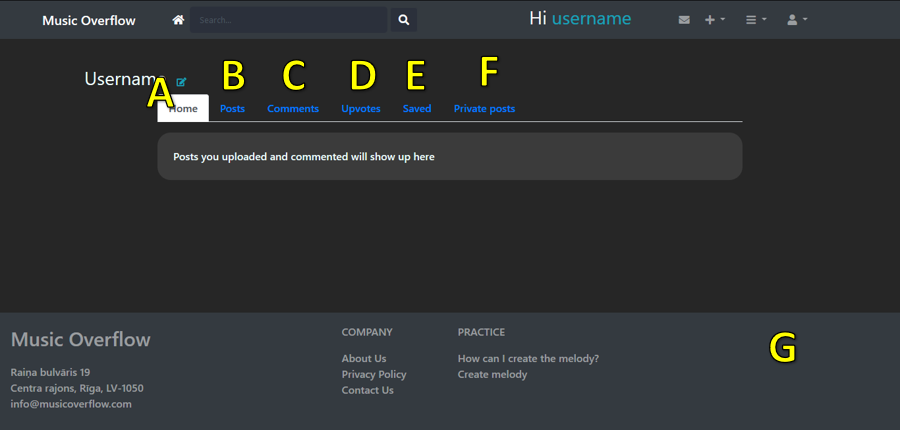
\includegraphics[scale=0.6]{profile.png}
	\caption{Lietotāja profils}
	\label{fig:profile}
\end{center}
\end{figure}

Lietotāja profila skatā (skat. ~\ref{fig:profile} attēlu) pieejamas šādas funkcijas:

\begin{itemize}
	\item A - Šeit tiks parādītas augšupielādētās un komentētās mūzikas atdarinājumi;
	\item B - Šeit tiks parādītas lietotāja izveidotās ziņas;
	\item C - Šeit tiks parādītas lietotāja komentētās ziņas;
	\item D - Šeit parādīsies ziņas, kurām lietotājs ir devis savu balsojumu;
	\item E - Šeit tiks parādītas saglabātās ziņas;
	\item F - Kājene, kas satur atgriezeniskās saites datus un citu informāciju, kas var būt noderīga lietotājiem.
\end{itemize}

\begin{figure}[H]
\begin{center}
	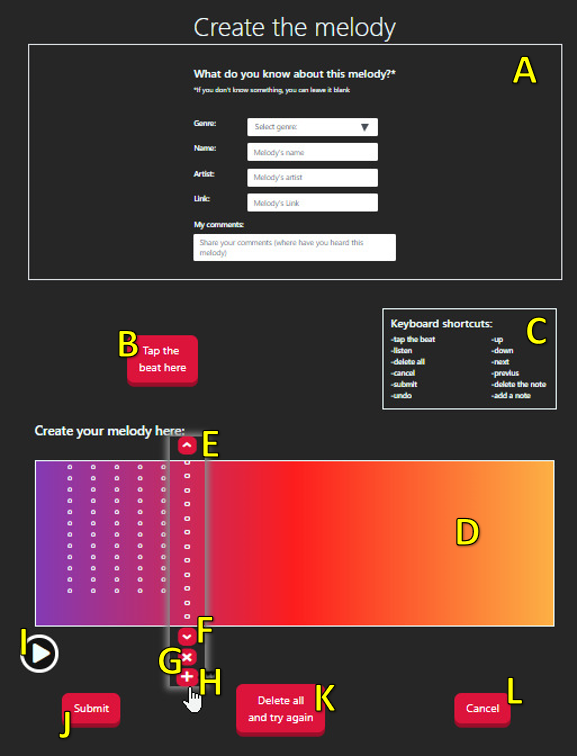
\includegraphics[scale=0.6]{melody.png}
	\caption{Melodijas izveide}
	\label{fig:melody}
\end{center}
\end{figure}

Melodijas izveidošanas skatā (skat. ~\ref{fig:melody} attēlu) pieejamas šādas funkcijas:

\begin{itemize}
	\item A - Šeit var norādīt informāciju par mūzikas atdarinājumu (nav obligāti);
    \item B - Šeit var pievienot bītus. Maksimālais mūzikas atdarinājuma intervals ir 10 sekundes;
    \item C - Šeit ir aprakstīti  taustiņu kombinācijas, kurus var izmantot mūzikas atdarinājuma veidošanai;
    \item D - Šeit var redzēt lietotāja izveidoto ritmu un notis;
    \item E - Pārvietot noti par vienu toni augšāk
    \item F - Pārvietot noti par vienu toni zemāk
    \item G - Dzēst noti
    \item H - Pievienot noti
    \item I - Klausīties mūzikas atdarinājumu;
    \item J - Izveidot mūzikas atdarinājumu;
    \item K - Dzēst visu izveidoto un sākt no jauna;
    \item L - Atgriešanās mājas lapā;
\end{itemize}

\begin{figure}[H]
\begin{center}
	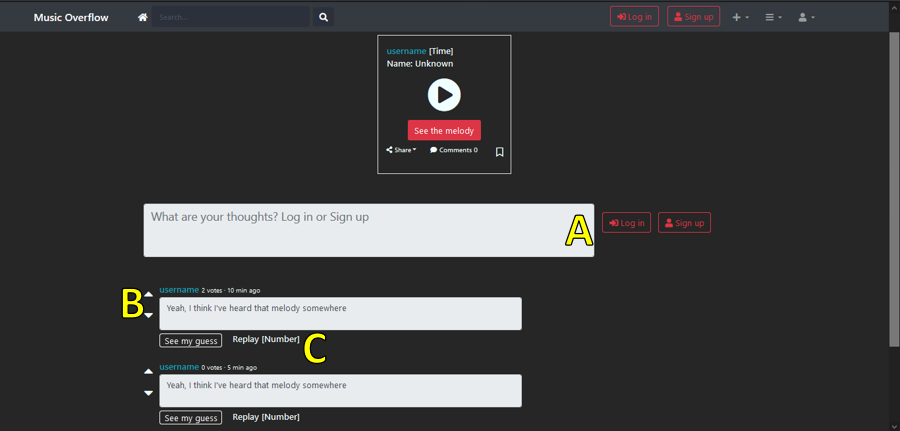
\includegraphics[scale=0.6]{comment1.png}
	\caption{Atbildes izveidošana}
	\label{fig:comment}
\end{center}
\end{figure}

Atbildes izveidošanas skatā (skat. ~\ref{fig:comment} attēlu) pieejamas šādas funkcijas:

\begin{itemize}
	\item A - Var uzrakstīt komentāru par mūzikas atdarinājumu, iepriekš pilnvaroties sistēmā, jo funkcija ir pieejama tikai pilnvarotiem lietotājiem;
    \item B - Var nobalsot par komentāru, izvēloties nospiest bultiņu uz augšu, kas nozīmē “+”, vai nospiest bultiņu uz lejū, kas nozīmē “-”, kas ietekmēs uz to, kādā vietā komentārs rādīsies. Jo vairāk komentāram “+”, jo augstāk tas rādīsies;
    \item C - Var atbildēt uz komentāru.	
\end{itemize}

\begin{figure}[H]
\begin{center}
	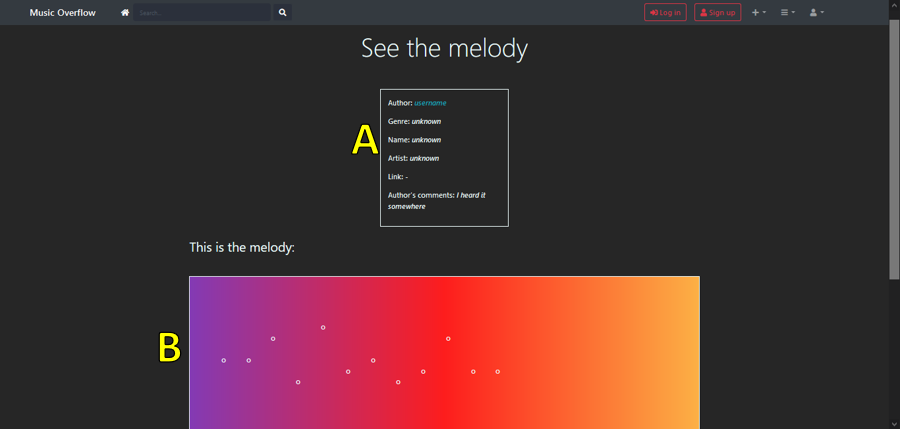
\includegraphics[scale=0.6]{seemelody.png}
	\caption{Melodijas apskatīšana}
	\label{fig:seemelody}
\end{center}
\end{figure}

Mūzikas atdarinājuma apskatīšanas skatā (skat. ~\ref{fig:seemelody} attēlu) pieejamas šādas funkcijas:

\begin{itemize}
	\item A - Informācija par mūzikas atdarinājumu (lietotāja, kas izveidoja mūzikas atdarinājumu, lietotājvārds, žanrs, nosaukums, dziedātājs, saite, lietotāja, kas izveidoja mūzikas atdarinājumu, komentārs)
	\item B - Var redzēt mūzikas atdarinājuma ritmu
\end{itemize}

\pagebreak

\section*{Izmantotā literatūra un avoti}
\addcontentsline{toc}{section}{Izmantotā literatūra un avoti}

\printbibliography

\pagebreak

\section{Pielikumi}

\centering \textbf{Pielikums 1. ``Mūzikas atdarinājuma izveides PPS''}
\begin{figure}[H]
\begin{center}
	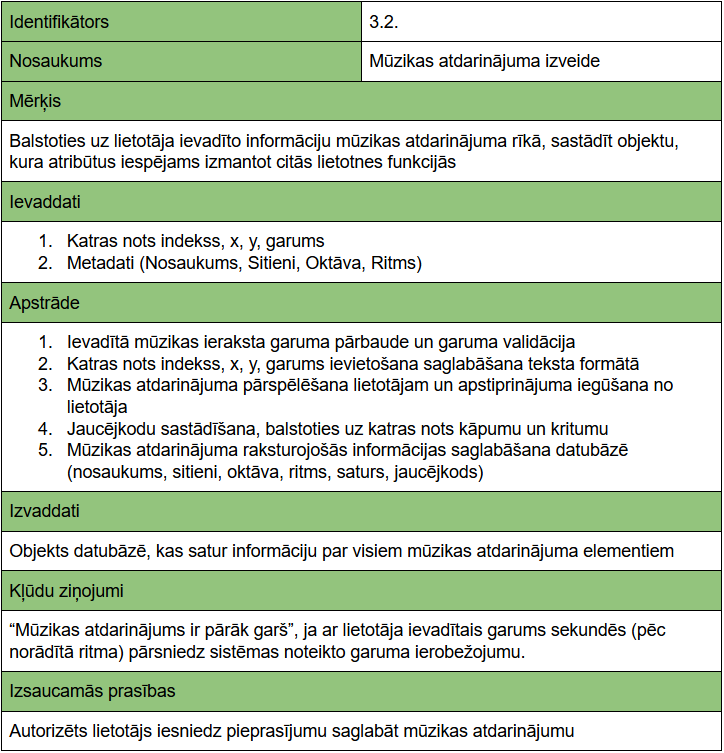
\includegraphics[scale=0.8]{Capture3.png}
	\label{fig:muzikasPPS}
\end{center}
\end{figure}

\pagebreak

\centering \textbf{Pielikums 2. ``Jautājumu rekomendācijas PPS''}
\begin{figure}[H]
\begin{center}
	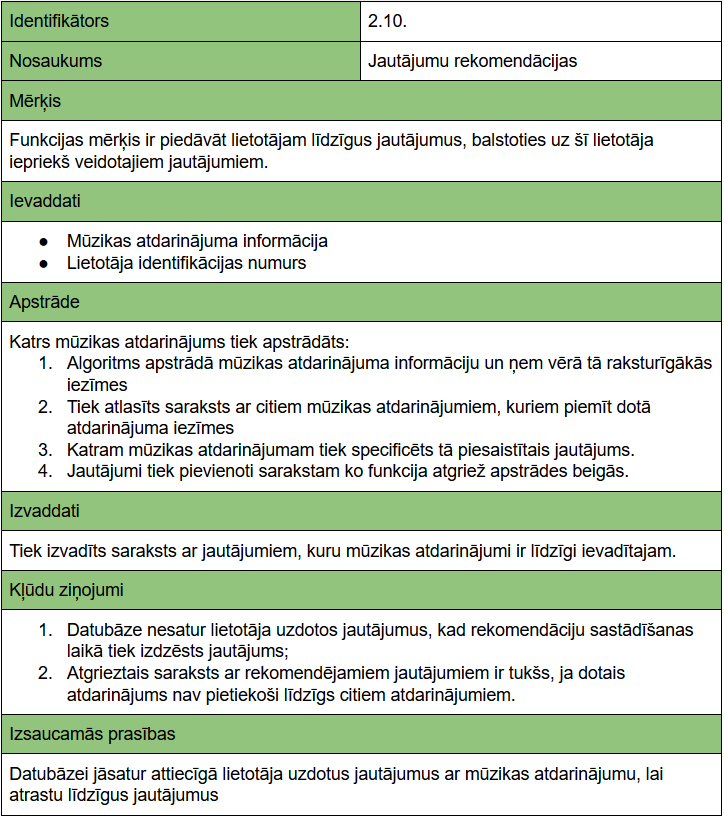
\includegraphics[scale=0.8]{Capture2.png}
	\label{fig:rekomendacijasPPS}
\end{center}
\end{figure}

\pagebreak

\centering \textbf{Pielikums 1. ``Atbilžu vērtēšanas PPS''}
\begin{figure}[H]
\begin{center}
	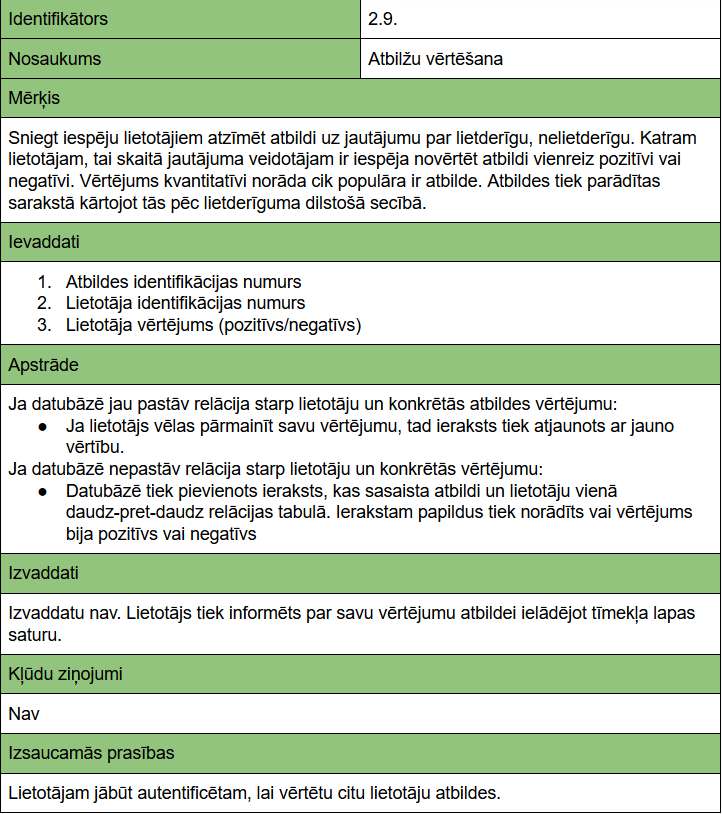
\includegraphics[scale=0.8]{Capture1.png}
	\label{fig:vertesanaPPS}
\end{center}
\end{figure}

\end{document}